\section{Model Comparison}\label{sec:comparisons}

\begin{figure*}
  \centering
  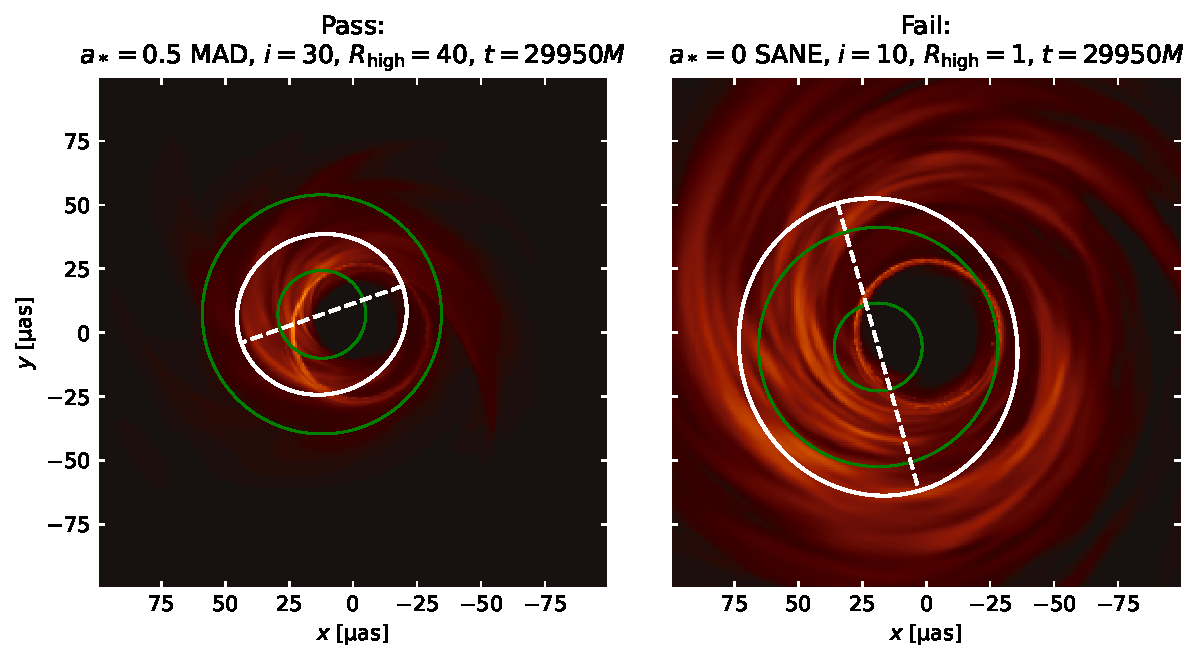
\includegraphics[height=3.25in]{figures/passfail_sz.pdf}
  \caption{Pre-image size constraint example.
    Left: passing snapshot;
    right: failing snapshot.
    The model is rejected if $< 1\%$ of model snapshots pass.
    The solid white ellipse  represents the second moments of the image, and the dashed line shows the major axis.
    The two green circles show the observed lower and upper limits from \citetalias{PaperIII}.
    The snapshot is rejected if the minor axis is larger than the upper limit, or if the major axis is smaller than the lower limit.}
  \label{fig:passfail_sz}
\end{figure*}

\begin{figure*}
  \centering
  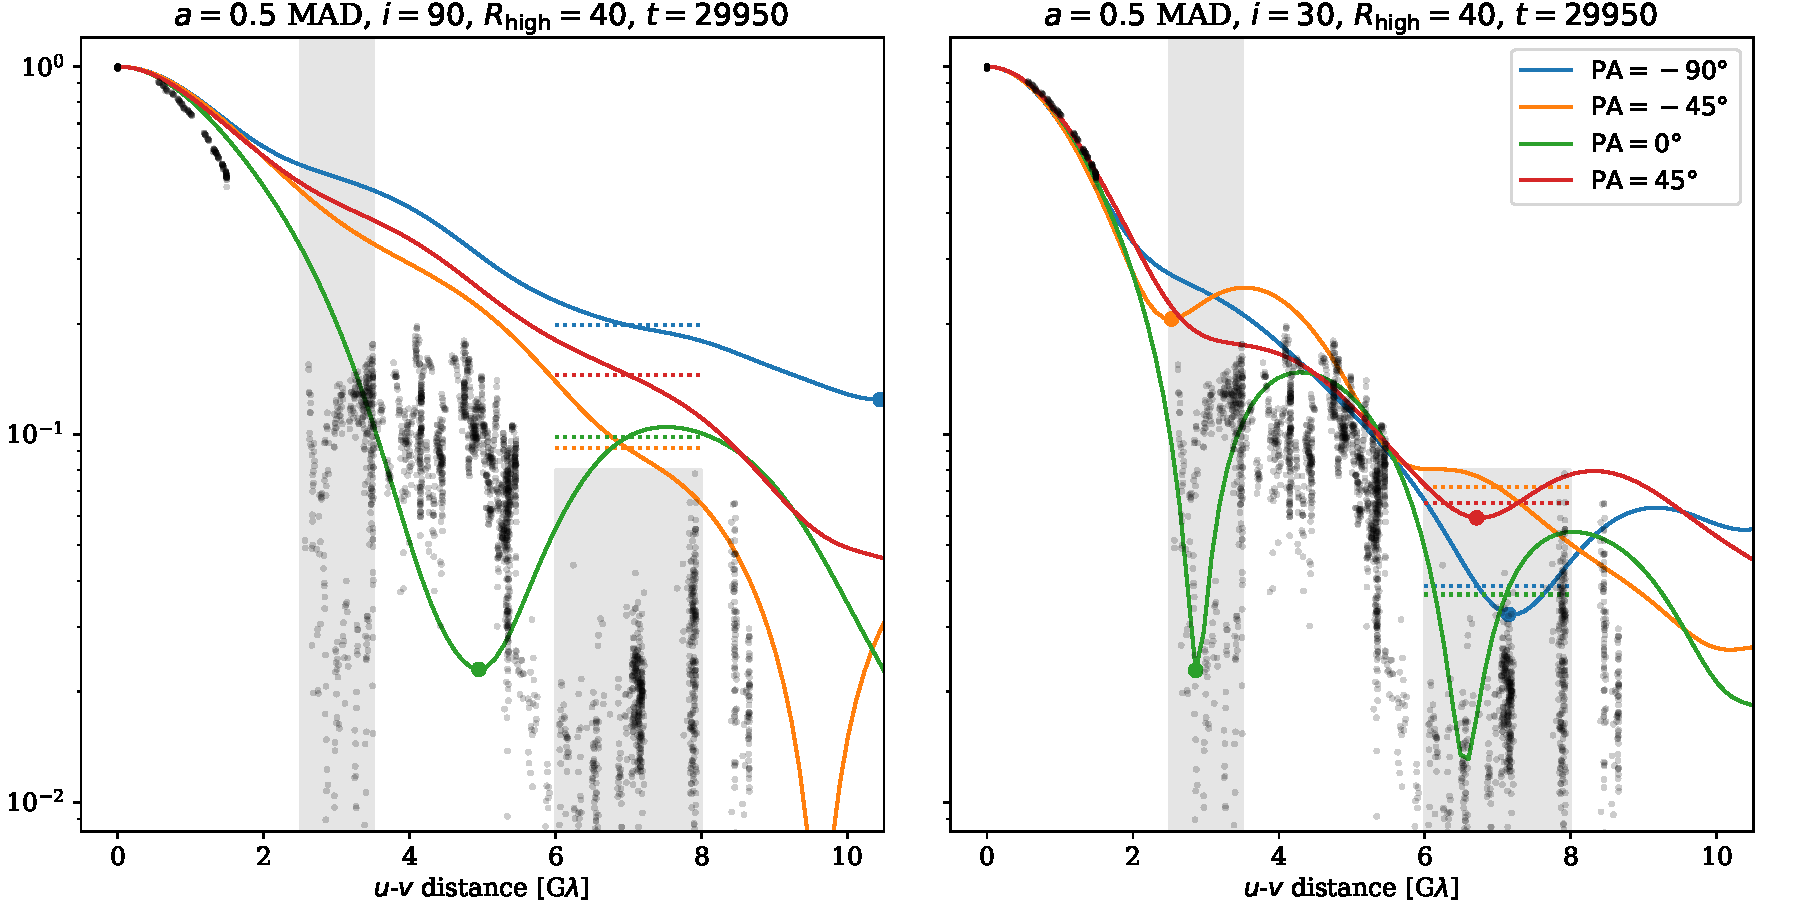
\includegraphics[height=3.25in]{figures/passfail_va.pdf}
  \caption{Visibility amplitude (VA) morphology  constraint example.
    \emph{Left}: passing snapshot;
    \emph{right}: failing snapshot.
    The solid lines in each plot show visibility amplitudes on a section through the origin in the \uv domain, at four position angles (PAs), where $0\degree$ is parallel to the projected angular momentum vector of the accretion flow.
    Solid black points show data from \aprilvii.
    The \vam constraint requires that for at least one PA the first minimum in VA fall within the left grey band, and for all PAs the median of the VAs lie inside the right grey band (see Section~\ref{sec:constraints}, \emph{Visibility Amplitude Morphology}, for details).
    Evidently the snapshot at right fails {\em both} conditions.}
  \label{fig:passfail_va}
\end{figure*}

\begin{figure*}
  \centering
  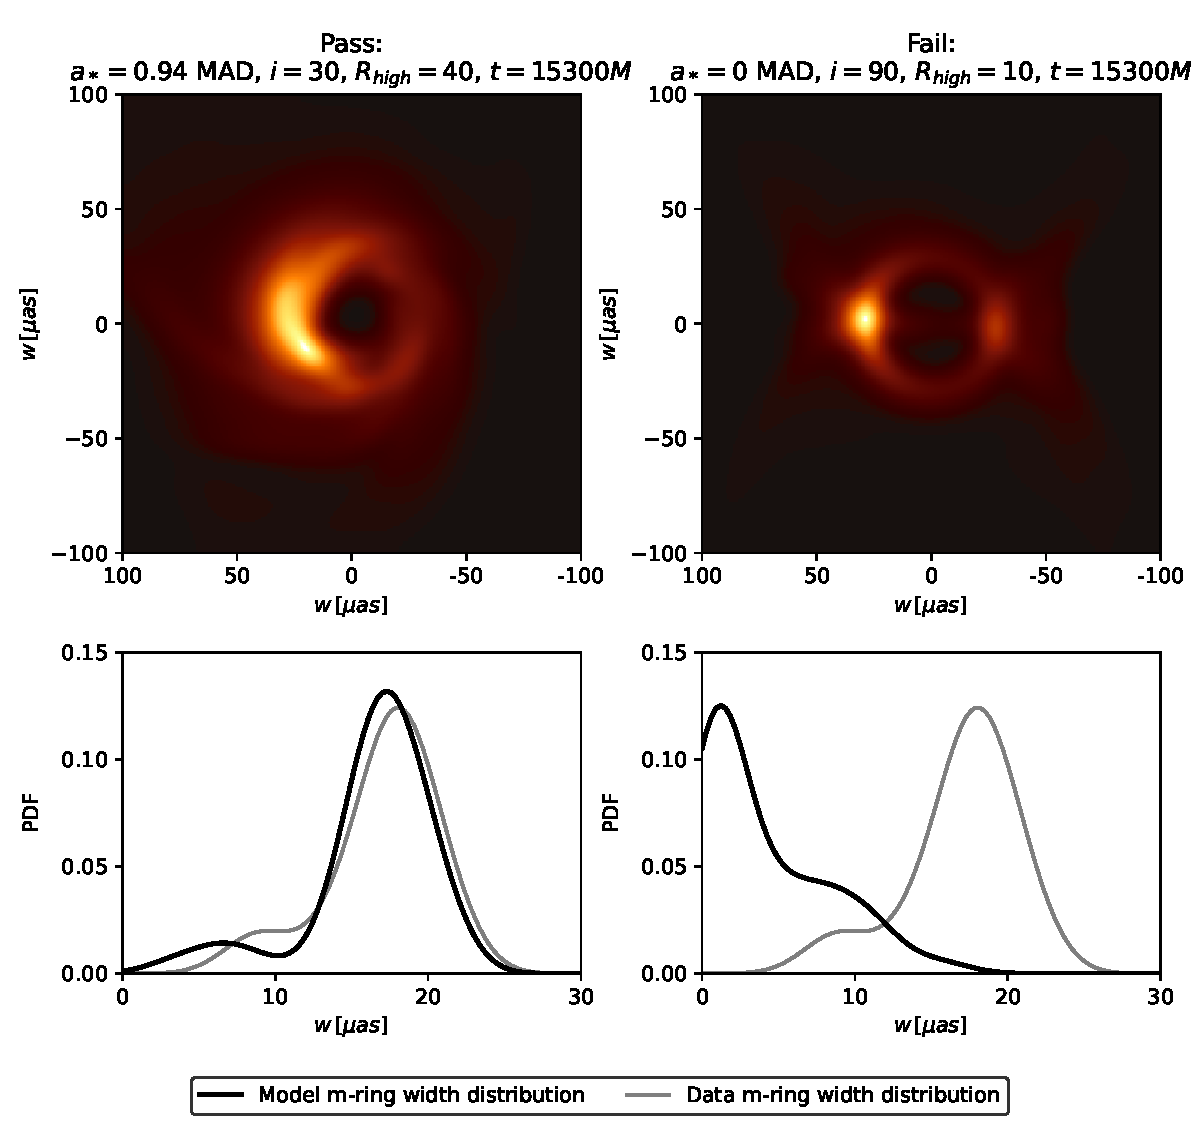
\includegraphics[width=0.75\textwidth]{figures/mring_width_example.pdf}
  \caption{\Mring width constraint example.
    \emph{Top left}: image that satisfies the constraint, Gaussian blurred to $20\uas$;
    \emph{top right}: image that fails the constraint;
    \emph{bottom left}: observed distribution of \mring widths over our 10 selected scans (light grey) and passing image distribution over 10 scans and 4 position angles (black);
    \emph{bottom right}: observed distribution of \mring widths over our 10 selected scans (light grey) and failing image distribution (black) over 10 scans and 4 PAs.}
  \label{fig:mring_width_example}
\end{figure*}

% cfg 2/5: I think this is unnecessary
%We now apply the observational constraints from Section~\ref{sec:observations} to the models described in Section~\ref{sec:models}.
%We have shown visually how models pass or fail in Figures~\ref{fig:passfail_sz}, \ref{fig:passfail_va}, and \ref{fig:passfail_sed}.
%For each of these figures, the left panel is from the best-bet region (see Section~\ref{sec:discussions}) that passes all but the variability constraints, and the right panel is one of the failed models.

%==============================================================================
\subsection{Fiducial Models}\label{subsec:thermal}

We start with the fiducial models.
Recall that these have aligned (prograde or retrograde) accretion flows, thermal eDFs, and electron temperature assigned according to the $\Rh$ model, as in \citetalias{M87PaperV}, and include the  \kharma, \bhac, and \hamr model sets listed at the top of Table~\ref{tab:radiativemodels}.

A set of plots showing how the three, redundant fiducial model sets fare for each constraint is provided in Appendix \ref{app:tables}.
Table~\ref{tab:passfraction_thermal} summarizes the fraction of fiducial \kharma, \bhac, and \hamr models that pass each constraint.

%------------------------------------------------------------------------------
\subsubsection{EHT Constraints}\label{sec:constraints}

% cfg 2/5: this also seemed redundant
%How do the models fare when compared to the EHT data alone, using the size, null location, and \mring fitting constraints?  The size constraint is simple but uninformative: only a few face-on, $\Rh = 1$ models fail the test.
%The null location test is informative and tends to rule out edge-on models.
%\Mring fits are noisy but informative---they are also consistent between model sets.
%Many fiducial models look like the data, but edge-on models are strongly disfavored.

%..............................................................................
\subsubsubsection{Second Moment}

Without assuming a ring, the EHT data allow a wide range of second moments.
The second moment constraint passes $98\%$ of all models.  Here and in what follows, the quoted passing fraction for the model describes the fraction of points in parameter space for which the existing model sets (\kharma, \bhac, and when present \hamr) agree that the model passes the constraint.
In short, nearly all fiducial models are about the right size once we use the 230\GHz to fix the mass unit $\mathcal{M}$.
The few rejected models are $\abh \le 0$, face-on, SANE models with $\Rh = 1$.
These models have extended emission on scales large compared to the critical impact parameter $b_c = \sqrt{27}\,\rg$.
The right panel of Figure~\ref{fig:passfail_sz} shows an example of one of these failed models.  The left panel shows an example of a passing model.

%..............................................................................
\subsubsubsection{Visibility Amplitude Morphology}
\label{sec:vam}

The \vam constraint tests the null location and long-baseline VAs.  Figure~\ref{fig:passfail_va} shows an example of a passing and failing model.
The constraint disfavors edge-on models at positive spin and a few large $\Rh$ SANE models.
This is mainly because the edge-on models contain bright spots, corresponding to the approaching side of the rotating accretion flow, and faint rings, so the first nulls get washed out by the bright features.
The \vam constraint passes 77\% of all models.

%..............................................................................
\subsubsubsection{\Mring Fits}

\begin{figure*}
 \centering
 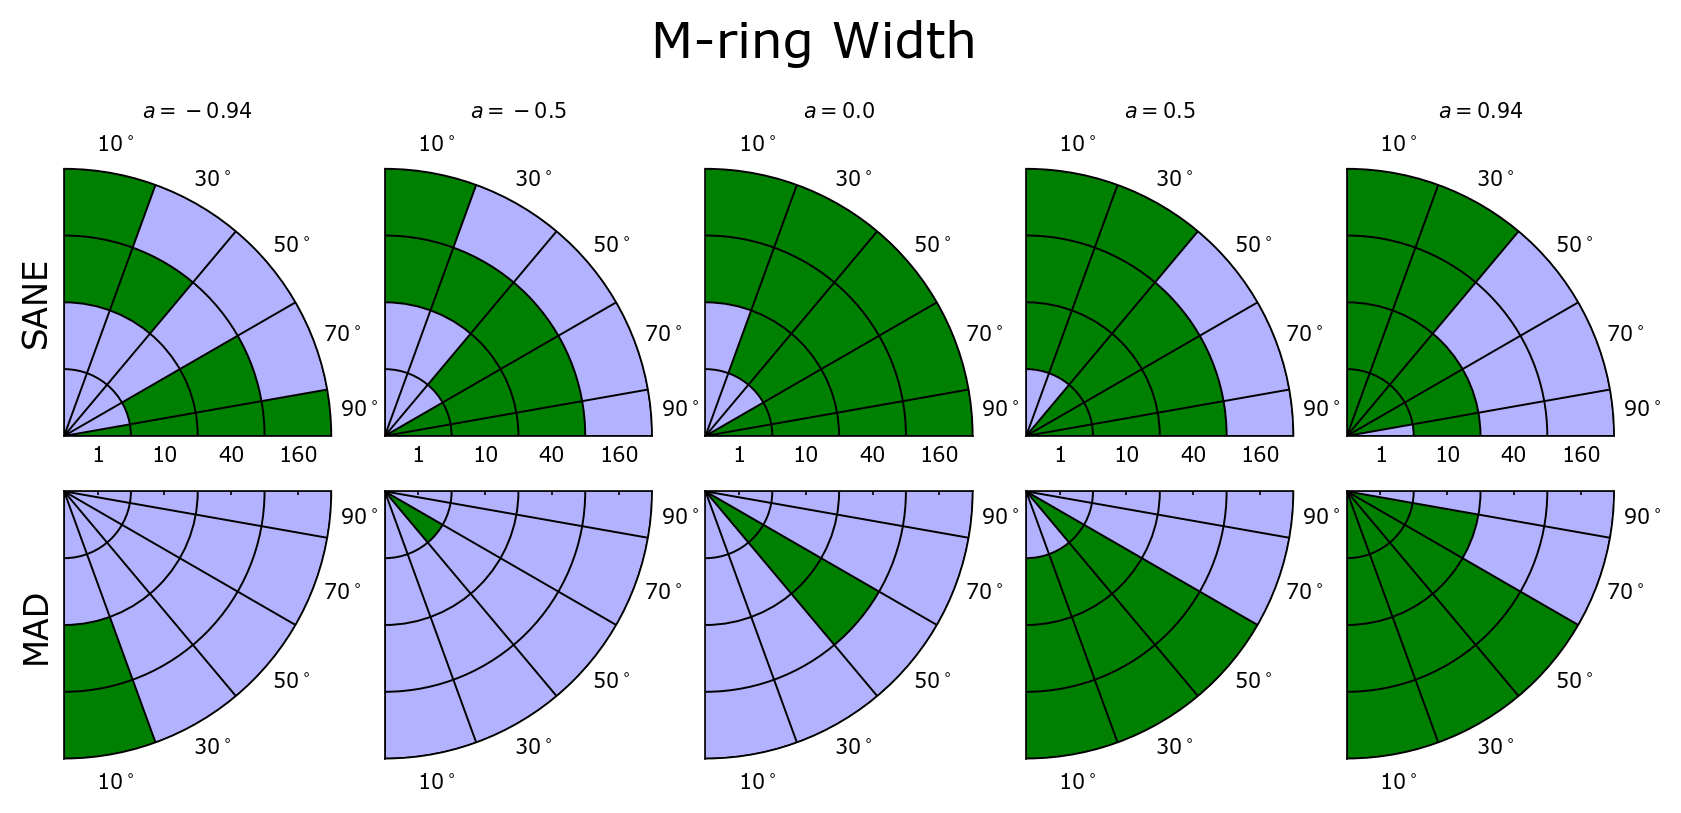
\includegraphics[width=\textwidth]{./figures/Mring_w_Constraints.png}
  \caption{Pass/fail plot for the \mring widths.
    Green indicates that the \kharma, \bhac, and \hamr models pass, yellow that one or two of the fiducial models fail, and red that all three fail.
    The inclination coverage is not uniform: \bhac and \kharma models cover all 5 inclinations while \hamr models cover $i = 10\degree$, $50\degree$, $90\degree$ only.
    The $i = 30\degree$, $70\degree$ wedges therefore include only the \bhac and \kharma models.}
  \label{fig:mring_width_salsa} % label must go after figure caption!
\end{figure*}

\begin{figure*}
  \centering
  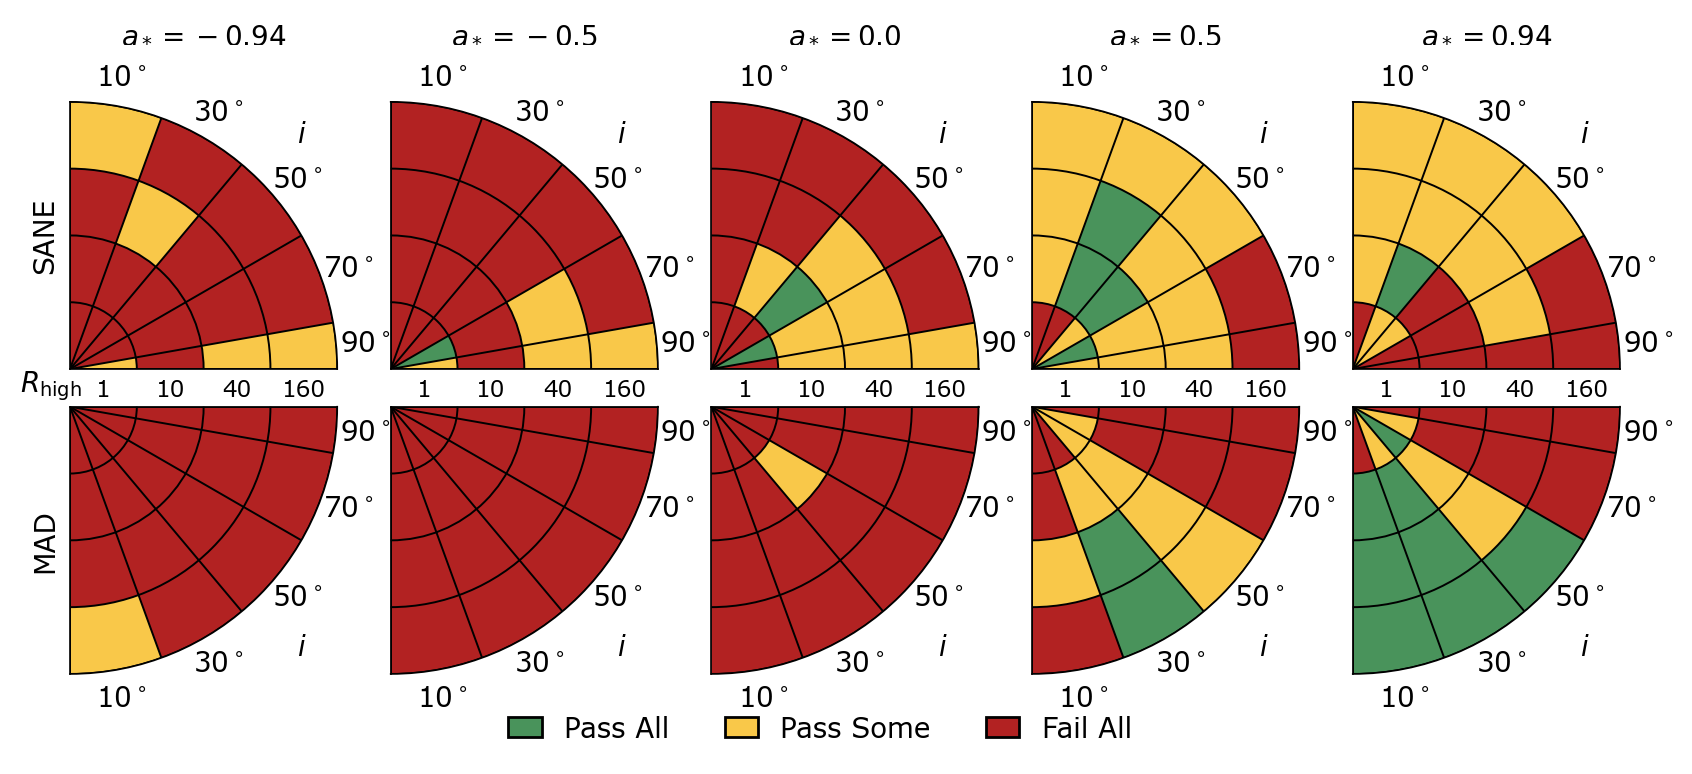
\includegraphics[width=\textwidth]{./figures/Interferometric_Constraints.png}
  \caption{Combined EHT constraints (logical {\em and}) including the second moment, \vam, and \mring fit constraints.
    Green indicates that the \kharma, \bhac, and \hamr fiducial models pass, yellow that one or two of the fiducial models fail, and red that all three fail.
    The inclination coverage is not uniform: \bhac and \kharma models cover all 5 inclinations while \hamr models cover $i = 10\degree$, $50\degree$, $90\degree$ only.}
  \label{fig:all_EHT_constraints} % label must go after figure caption!
\end{figure*}

The \mring asymmetry, diameter, and width are treated as separate constraints.
Recall that we compare the distribution from the data to that from the model using a two-sample KS test.

The asymmetry parameter is typically not well constrained.
Many rejected models are at high inclination and have $\abh =0.94$.
These models have asymmetries that are large and detectable because Doppler boosting concentrates emission in an equatorial spot on the approaching side of the disk.
The asymmetry parameter constraint passes 90\% of all models.

The \mring diameter, which depends on the diameter of the shadow and the ring width, is better constrained than the asymmetry parameter and varies systematically from model to model.  %The rejected models tend to be low inclination models at negative $\abh$.
%For example, the distribution of diameters is much broader at $\Rh = 1$ than at larger values of $\Rh$.
The ring diameter constraint passes 55\% of all models.

Most of the models that fail are low inclination models with ring diameters that are too large. Only two \bhac models fail because the ring diameter is too small.  Most of the rejected models are low inclination models at $\abh < 0$.
%For example, the $i = 10\degree$, $\Rh = 10$ SANE models fail for all spins with $\abh \le 0$ because the ring is too large.
%The same is true for all $i = 10\degree$ MAD models with $\Rh = 1$.

%The distribution of \mring diameters for many SANE models is multimodal (consistently so in the fiducial model sets), with a secondary peak in the distribution at $\sim 35\uas$.
%%All $\Rh = 1$ SANE models show this secondary peak.
%The images of these models tend to have a well defined ring at the critical impact parameter and a second broad maximum in intensity at larger impact parameter.
%The second peak in the distribution is a consequence of limited baseline coverage.

The \mring width $w$ is the most tightly constrained of the three \mring parameters.
Although the closure phases constrain $w$ as well, it is easiest to see how $w$ affects visibility amplitudes at long baselines.
For example, for a circularly symmetric ring the VAs are a Bessel function multiplied by a Gaussian with width $\sim 1/w$.  Increasing $w$ therefore decreases the amplitude of the long baselines.
Figure~\ref{fig:mring_width_example} shows examples of models that pass and fail the \mring width constraint.

Figure~\ref{fig:mring_width_salsa} summarizes the pass/fail status of the fiducial models for the \mring width.
All rejected models have median $w$ that is below the median of the data, $ \simeq 17.5\uas$.
The rejected models include all MAD models at $\abh \le 0$ and all edge-on ($i = 90\degree$) models in the \kharma, \bhac, and \hamr fiducial models.
MAD models exhibit a strong trend toward smaller $w$ as $i$ increases.
SANE models exhibit a similar but weaker trend.
The SANE model images have  higher optical depth, broader rings, and more substructure than the MAD models.
Their $w$ distributions are typically broad, with mode well below $17.5\uas$.
Only for $\abh = 0.94$, where the optical depth is lower due to higher temperatures in the emitting region, do most of the models exhibit a sharply peaked $w$ distribution centered at $17.5\uas$.

%..............................................................................
\subsubsubsection{EHT Constraint Summary}

We can combine all EHT constraint cuts with a logical {\em and} operation.
The results are summarized in Figure~\ref{fig:all_EHT_constraints}.
Evidently EHT data alone are capable of discriminating between models.
The edge-on ($i = 90\degree$) models all fail, with some failing \mring width, diameter, asymmetry and the \vam  constraint.
The cuts clearly favor $\abh > 0$ models, with a few exceptions.
There are two clusters of models that do not fail any constraints in any models: positive spin MAD models at low inclination, and positive spin SANE models, also at low inclination.

%------------------------------------------------------------------------------
\subsubsection{Non-EHT Constraints}

\begin{figure*}[h!]
  \centering
  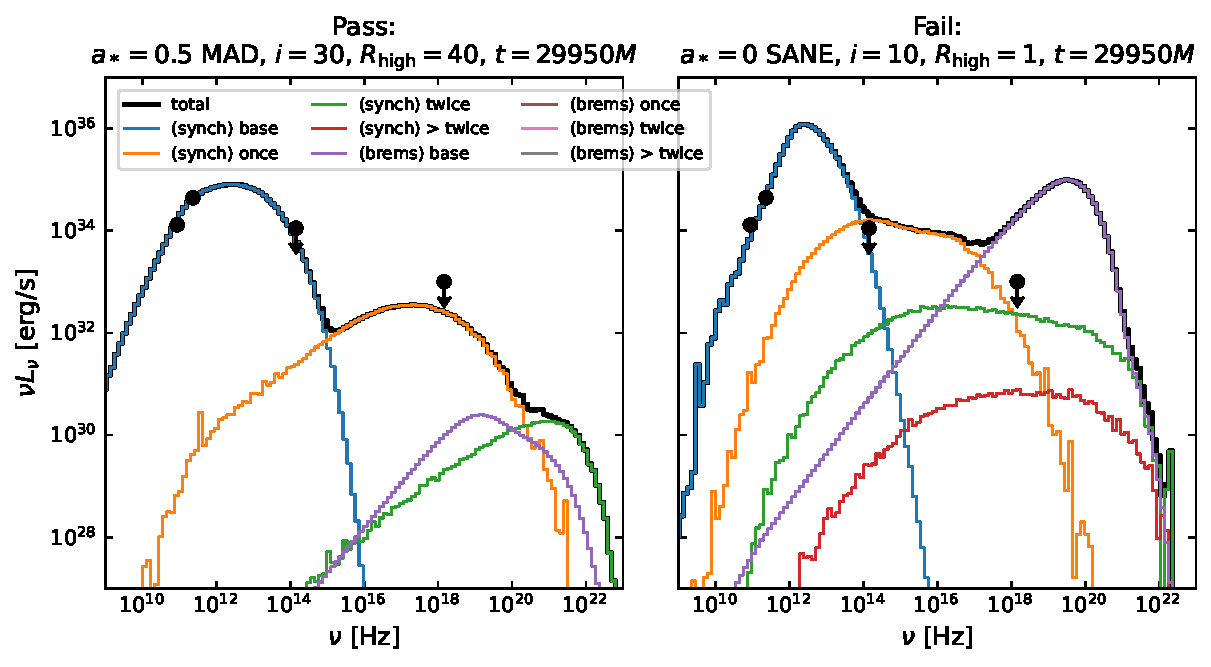
\includegraphics[height=3.25in]{figures/passfail_sed.pdf}
  \caption{%
    Non-EHT flux density constraint example.
    \emph{Left}: passing model with SED close to the measured 86\GHz point and below the quiescent $2.2\um$ and X-ray points.
    \emph{Right}: failing model with inconsistent (strongly rising) millimeter wavelength spectral index, overproduction of $2.2\um$ due to strong Comptonization, and overproduction of X-rays by bremsstrahlung.}
  \label{fig:passfail_sed}
\end{figure*}

\begin{figure*}
  \centering
  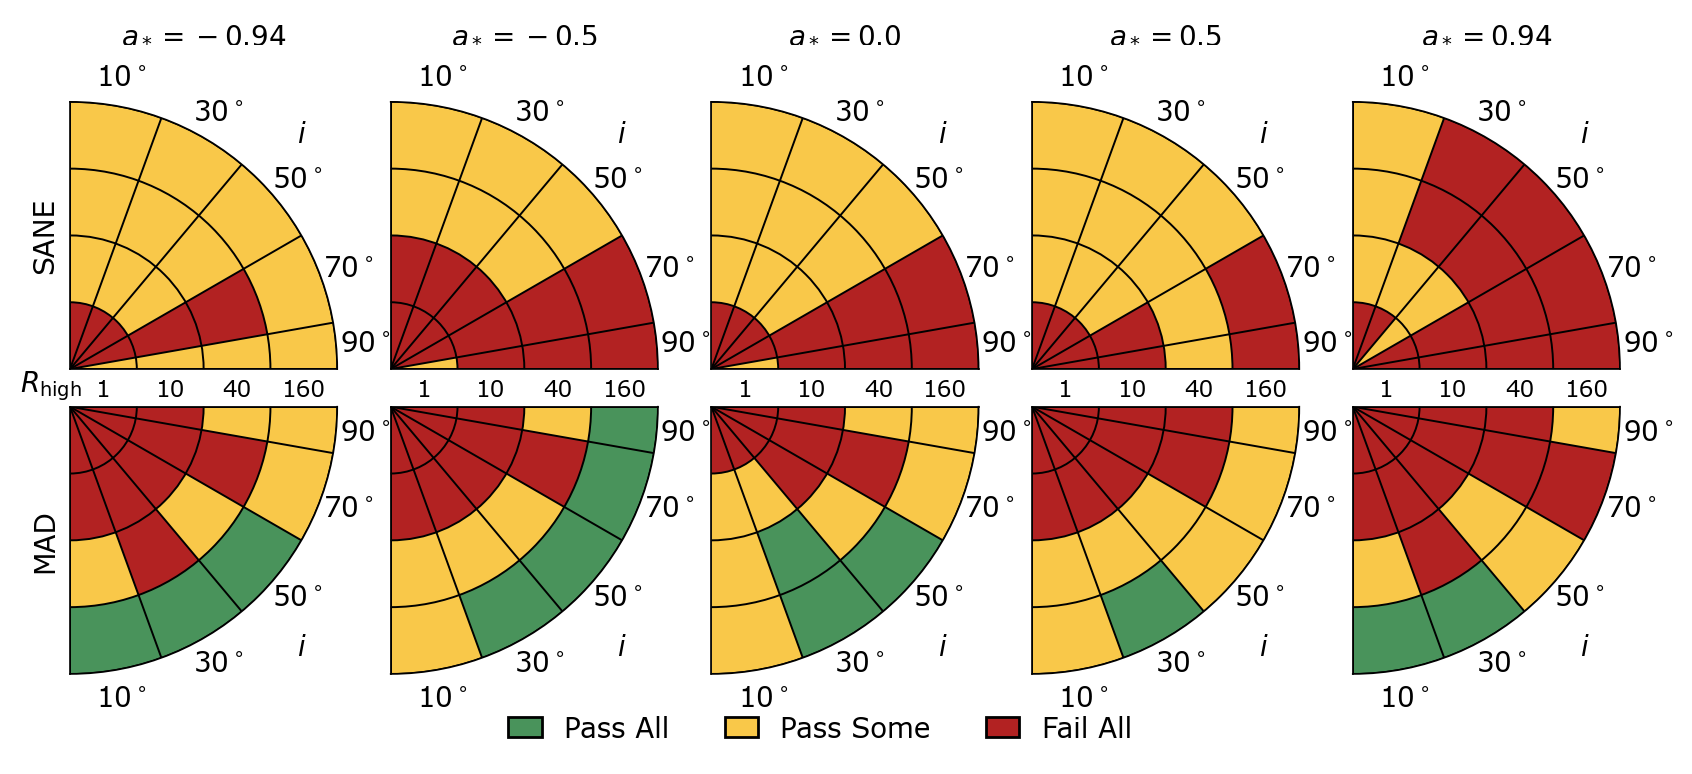
\includegraphics[width=\textwidth]{./figures/Non_Interferometric_Constraints.png}
  \caption{Combined non-EHT constraints (logical {\em and}).
    Green indicates that the \kharma, \bhac, and \hamr models pass, yellow that one or two of the fiducial models fail, and red that all three fail.}
  \label{fig:non_eht_cuts}
\end{figure*}

% cfg 2/5: this is not necessary
%We now consider constraints from unresolved $86\GHz$, $2.2\um$, and X-ray
%observations.
%Some or all of the emission in these bands are believed to originate
%in the compact source from plasma that is close to or overlaps the
%plasma that is producing the 230\GHz-emitting plasma observed by EHT.
%Figure~\ref{fig:noneht_pizza} in the appendix shows which models
%pass and fail these constraints in aggregate.

%..............................................................................
\subsubsubsection{86\,GHz Flux Density}

In a simplified picture \sgra's millimeter flux is produced in a photosphere that decreases in size as frequency increases.
Because optical depth is not large at 230\GHz ($\sim 0.4$ in the one-zone model) and the source structure is complicated (the optical depth varies across the image) the simplified picture is imprecise.
Nevertheless 86\GHz emission is on average produced at larger radius than 230\GHz emission, and the 86\GHz source size is larger than the 230\GHz source size.  The ratio of 86\GHz to 230\GHz flux density is therefore sensitive to the radial structure of the source plasma.

Figure~\ref{fig:86GHz_flux_pizza} records the results of applying this constraint.
Most $\Rh = 1$ models, both MAD and SANE, fail the 86\GHz flux density test.
The 86\GHz flux density is quite sensitive to $\Rh$.
For example, SANE $\abh = 0.5$, $i = 70\degree$, $90\degree$ models are too bright at $\Rh = 1$ and too dim at $\Rh = 10$.  This suggests that there are passing models in between, and that the parameter space is not sampled densely enough.
Finally, the 86\GHz flux constraint strongly favors MAD models over SANE models in all three fiducial model sets.

%..............................................................................
\subsubsubsection{86\,GHz Major Axis}

As for the 86\GHz flux, the 86\GHz size is sensitive to optical depth as a function of radius in the source plasma.
Figure~\ref{fig:86GHz_size_pizza} in Appendix~\ref{app:tables} shows the full results of applying this constraint.

The 86\GHz size is sensitive to inclination.
For example, the SANE, $\abh = 0$, $\Rh = 40$ models are too small at low inclination and too large when seen edge-on, because the edge-on models have prominent limb-brightened jet walls that are visible to $100\uas$.
The 86\GHz size constraint passes only $58\%$ of models and is therefore one of the tightest constraints.

The physical picture for 86\GHz source size is complicated, as is the extraction of the constraint itself from observations.
Notice that
\emph{i})~two different values for the 86\GHz intrinsic source size have been reported in the literature (see Section~\ref{sec:86size});
\emph{ii})~scattering is $7$ times stronger at 86\GHz than at 230\GHz;
\emph{iii})~scattering must be subtracted accurately to obtain the intrinsic source size; and
\emph{iv})~the error bars for the 86\GHz source size are narrow and this plays a key role in determining the strength of the constraint.
%\footnote{Comparing the 86\GHz major axis and 230\GHz second moment constraints, it may seem surprising that 230\GHz has much larger range.
%This is \emph{not} due to, e.g., measurement uncertainty in the visibility.
%Instead, it is because the more complicated source structure at this 230\GHz.
%See Section~5.1.3 in \citealt{PaperII} for details.}

%..............................................................................
\subsubsubsection{\texorpdfstring{$2.2\um$}{2.2um} Median Flux Density}

$2.2\um$ photons are produced by the synchrotron process from electrons on the high energy end of the eDF.
For the one-zone model with $B = 30$\,G and $\Theta_e = 10$, the mean Lorentz factor is $\gamma = 30$ and the synchrotron critical frequency $\nu_\mathrm{crit} = \gamma^2 e B/(2 \pi m_e c) \simeq 80\GHz$.
Emission at $2.2\um$ is produced by electrons with Lorentz factor $\gamma \simeq 10^3$, so $2.2\um$ flux density is sensitive to $\Theta_e$ and $B$.
Both increase toward the horizon, and field strength is nearly independent of latitude, so $2.2\um$ photons are produced at small radius in regions where $\Theta_e$ is highest.

The sensitivity to $\Theta_e$ implies that $2.2\um$ flux density will be highest for models with higher temperatures.
For SANEs the midplane gas temperature, and therefore electron temperature in the $\Rh$ prescription, increases with $\abh$, so the highest $2.2\um$ flux density is at positive $\abh$.

The sensitivity to $B$ implies that $2.2\um$ flux density will be highest for parameters with stronger fields.  $B$ depends on the GRMHD flow configuration and also on the accretion rate, which is fixed by the observed $F_{230}$, so when all else is equal the $2.2\um$ flux density is highest when the accretion rate is largest.  The dependence of accretion rate on model parameters is discussed in Section~\ref{sec:accrate_outflowpower}.  In brief, for SANE models the accretion rate declines as $\abh$ increases and $\Rh$ decreases. For MAD models the accretion rate dependence on $\abh$ and $\Rh$ is relatively weak.

Finally, the $2.2\um$ flux density is also sensitive to inclination.  A combination of Doppler boosting and the rapid falloff in emissivity in the NIR means that at large inclination lower frequency emission from the approaching side of the accretion flow is boosted into the NIR and thus $2.2\um$ flux is higher at high inclination.
%the Doppler effect (blueshift) enables photons that are detected at $2.2\mu$m to be emitted at longer wavelength, where the emissivity is usually larger, in plasma that is moving toward the observer, and the accompanying Doppler beaming increases the detected intensity.
%We therefore expect $2.2\um$ flux density to increase with inclination and to peak in the midplane on the approaching side of the flow.

Models that pass the $2.2\um$ flux limit are shown in Appendix~\ref{app:tables} in Figure~\ref{fig:2um_flux_pizza}.
The rejected SANE models ($7\%$ rejected by all of \kharma, \bhac, and \hamr) tend to be at high inclination: their images are dominated by a bright spot on the approaching side of the disk.
The rejected MAD models ($53\%$) include nearly all models at $\Rh = 1$ and $\Rh = 10$, where $\Theta_e$ tends to be larger, and the majority of high-inclination models, where the effect of Doppler boosting is largest.

We find that some models are Compton dominated at $2.2\um$.
For example, $\abh = -0.94$ SANE models become optically thin at relatively low frequency as $\Rh$ goes to $1$, and thus synchrotron emission drops off rapidly as frequency increases.  When the synchrotron is weak enough the underlying bump of Comptonized millimeter photons dominates.
%As $\Rh$ drops and synchrotron decreases the SED becomes dominated by a lower-luminosity bump of underlying Comptonized photons.
%Just before this happens, at $\Rh = 10$, the combination of the Compton bump and synchrotron emission is enough to push the median $2.2\um$ flux density above the observational limit, explaining the excluded SANE models at $\Rh = 10$, $\abh = -0.94$.

%..............................................................................
\subsubsubsection{X-ray Luminosity}

X-ray production in fiducial models is typically dominated by Compton upscattering of thermal synchrotron photons.
In the first Compton bump $\nu L_\nu$ is thus proportional to the y-parameter $y \sim 16 \Theta_e^2 \tau_e$ where $\tau_e$ is a characteristic electron-scattering optical depth and $\Theta_e$ is a typical dimensionless electron temperature.
At $\Rh = 1$ the X-ray band lies in the first Compton bump, while at larger $\Rh$ the bumps move to lower energy because the bulk of the Thomson depth is in the midplane where $\Theta_e \propto 1/\Rh$.

We find that in a few large $\Rh$ SANE models, however, X-ray emission is dominated by bremsstrahlung (synchrotron never dominates the X-ray in thermal models).  Bremsstrahlung emissivity $j_{\nu,b} \propto n^2$, so at fixed temperature bremsstrahlung increases rapidly with density. Notice that $j_{\nu,b} \propto \Theta_e^{1/2}$ for $\Theta_e > 1$ and $\Theta_e^{-1/2}$ for $\Theta_e < 1$, so cool disks enhance bremsstrahlung.  Bremsstrahlung therefore dominates Compton in models with high density and low temperature, which happens in models with large $\Rh$ (see Section~\ref{sec:discussions}).  We note that bremsstrahlung emission arises at larger radii than the synchrotron and Compton-upscattered X-ray emission and therefore varies more slowly.

The X-ray cuts are shown in Appendix~\ref{app:tables},  Figure~\ref{fig:xray_pizza}.  Some large $\Rh$ SANE models fail due to excess bremsstrahlung, although there is notable disagreement between \bhac and \kharma for SANE X-ray fluxes.
MAD models that fail have low $\Rh$ and are Compton-dominated in the X-ray.
Nearly all $\Rh = 1$ MAD models fail the X-ray constraint, as do many at $\Rh = 10$.  This is because the midplane $\Theta_e$ increases as $\Rh$ goes to $1$.
Since the midplane contributes most of the electron scattering optical depth, low $\Rh$ models have the largest $y$ parameter and are at greatest risk of overproducing X-rays.
%\michi{Need to update this explanation to reflect contradicting \bhac results}

%..............................................................................
\subsubsubsection{Summary of Non-EHT constraints}

Applying only non-EHT constraints $7\%$ of models as shown in Figure~\ref{fig:non_eht_cuts}.
The surviving models are the result of applying a heterogeneous and noisy set of constraints using a hard cutoff, which somewhat obscures the underlying physical picture.
Nevertheless, the surviving 13 models are all MAD and all have $\Rh > 10$.  All but two have $i < 70\degree$.
This leaves a cluster of surviving MAD models at large $\Rh$ and low to moderate inclination.

%------------------------------------------------------------------------------
\subsubsection{Variability}

\begin{figure}
  \centering
  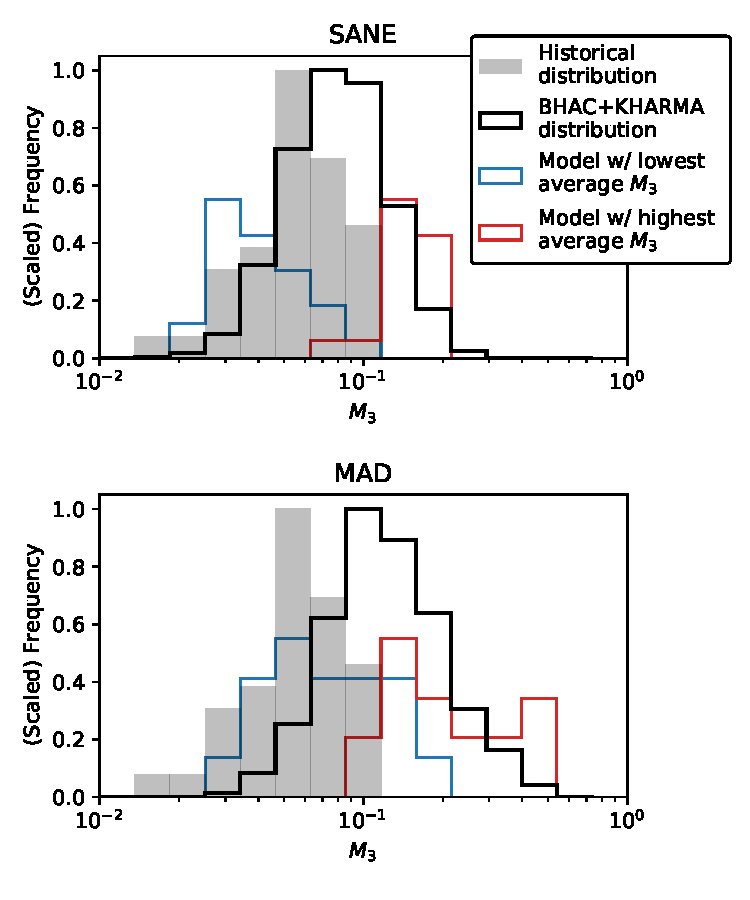
\includegraphics[width=\columnwidth]{./figures/mi_hist.pdf}
  \caption{Distributions of 3-hour modulate index $\mi{3}$ for \bhac, \kharma, and \hamr models (black), compared to distributions from historical observations (gray).
The distributions for models with the lowest (blue) and highest (red) average $\mi{3}$ for SANEs and MADs are also shown.
The heights of these distributions have been scaled for clarity.}
  \label{fig:cmp_ALMA_var}
\end{figure}

Variability is central to the interpretation of EHT observations of \sgra: an $8\,\mathrm{hr}$ observation of \sgra lasts $\no{1400}\,\tg$, a timescale over which most models vary substantially.
In contrast, an $8\,\mathrm{hr}$ observation of M87* is $\sim \tg$ and on this timescale M87* hardly varies at all.

% cfg 2/5: this par doesn't add anything
%Variability is a strong constraint.
%Although models differ in their degree of variability, both in an integrated sense and on 2--6~$G\lambda$ baselines, only a small fraction of models are as quiet as the data.
%For the light curve variability, this remains true whether we use data from April~7, 2017, all days from the 2017 observing campaign, or from historical monitoring of \sgra.
%In general, we find that SANE models are quieter than MAD models, and (to a lesser extent) face-on models are quieter than edge-on models.

Recall that we consider two variability constraints, one on the 230\GHz light curve and the other on 230\GHz VAs.  We find that SANE models are less variable than MAD models. Only 3.5\% of models, all SANE, pass both variability constraints.  A possible interpretation of this result is that the models are missing a physical ingredient that would reduce variability, and this is discussed in Section~\ref{sec:discussions}.
%One interpretation is that there is a missing physical ingredient in the models, which could affect our entire model library.  This possibility is discussed in Section~\ref{sec:discussions}.

%..............................................................................
\subsubsubsection{Modulation Index}

The distribution of 3-hour modulation index ($\mi{3}$) across all fiducial SANE models, across all fiducial MAD models, and across the historical dataset are shown in Figure~\ref{fig:cmp_ALMA_var}.
The plot also shows distributions for individual models with the lowest and highest median $\mi{3}$.

The $\mi{3}$ cuts are summarized in Appendix \ref{app:tables}, Figure~\ref{fig:m3_pizza}.
We find that:
\emph{i})~as a group, the fiducial models are more variable than the data;
\emph{ii})~the MAD models are more variable than SANE models;
\emph{iii})~eleven individual models  pass the constraint for all fiducial model sets, and these are exclusively SANE models;
\emph{iv})~there are some differences between variability in the fiducial model sets, with \hamr models notably more variable than \kharma and \bhac models; and
\emph{v})~the pass fractions for the fiducial model sets are 20\% for \kharma, 27\% for \bhac, and 7\% for \hamr.
The modulation index is the tightest single constraint on the models.

%..............................................................................
\subsubsubsection{4 \texorpdfstring{$G\lambda$}{Gl} Visibility Amplitude Variability}

\begin{figure}
  \centering
  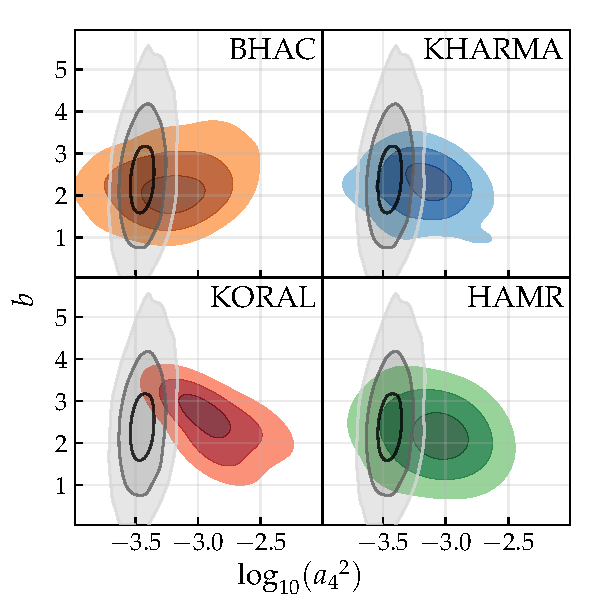
\includegraphics[width=\columnwidth]{./figures/grmhd_triangle_debiased_combined.pdf}
  \caption{Distributions of $(\log_{10}(\afour^2), b)$ for \bhac, \kharma, \koral, and \hamr, compared against the 2017 EHT confidence regions (gray).}
  \label{fig:cmp_VLBI_var}
\end{figure}

The power-law index $b$ of the variance $\sigma_\text{var}^2 (|u|)$ at 2--6\,G$\lambda$ of the models is generally in good agreement with the value measured  from the 2017 EHT campaign (excluding April 11).
The amplitude $\afour^2$, however, varies depending on the model.

Figure~\ref{fig:cmp_VLBI_var} shows the distribution of $(\afour^2, b)$ from the EHT observation, along with the distributions across all fiducial models.
For a single model, the number of measurements of $(\afour^2, b)$ is equal to the number of windows for that model (three in most cases).  The \koral models appear more variable because they include only $\Rh = 20$ MAD models at various spins.  

The models tend to be more variable than the observations, with face-on models performing better than edge-on models.
For SANE models, $\Rh = 10$ tends to be more variable than others.
For MAD models, there is a slight preference for lower $\Rh$.

\subsubsubsection{Long duration \koral models}

We have imaged a set of MAD models run with the \koral code out to $\sim \no{100000}\,\tg$.  These long duration  models have $\Rh = 20$, which lies off our fiducial model parameter grid.  They enable us to assess the importance of integration time for application of the constraints, and provide a more accurate distribution for, e.g. \mi{3}.  

The \koral models are discussed in Appendix~\ref{app:variability}. In brief we find no evidence for significantly different variability when comparing the first and second half of the \koral runs, consistent with no long-term evolution of the variability.  We also find no significant differences when comparing the \koral runs to nearby models on the fiducial model parameter grid.  Notice that in Figure \ref{fig:cmp_VLBI_var} the \koral models are more variable than the other model sets only because the other model sets contain lower-variability SANE models.

%These long duration models enable us to assess the importance of integration time for application of the constraints.
%They also provide a more accurate distribution for the constraint quantities and to assess whether the constraints evolve from the beginning to end of the integrations.
%We do not see evidence for evolution in the \koral model set (a full pass/fail table is given in Appendix~\ref{app:tables}
% Table~\ref{tab:koralPF} %% OUCH... the table is not used in the latest version
%and more detailed discussion in Appendix~\ref{app:variability} and in \citealt{Georgiev_2022}).
%The \koral pass/fail results are similar to those for comparable models in the fiducial model sets.
%Moreover the constraints measured at the beginning of the evolution are similar to those measured at the end.

%------------------------------------------------------------------------------
\subsubsection{Summary of Constraints on Fiducial Models}
\label{sec:summarythermal}

\begin{table*}
\caption{Summary of constraints and passing fractions for \kharma, \bhac, and \hamr thermal models}
\centering
\begin{tabular}{l|l|ccc}
\hline
Constraint & Description & \kharma	&	\bhac	&	\hamr \\
\hline
230\,GHz size	        &	&	0.98	&	0.98   &	1.0		\\
lc varability	        &	&	0.20	&	0.27   &	0.07	\\
4G$\lambda$ variability	&	&	0.60	&	0.72   &	0.39	\\
Null location	        &	&	0.84	&	0.83   &	0.80	\\
M-ring diameter	        &	&	0.67	&	0.65   &	0.61	\\
M-ring width	        &	&	0.35	&	0.21   &	0.32	\\
M-ring asym.	        &	&	0.94	&	0.95   &	0.99	\\
86\GHz size	            &	&	0.62	&	0.59   &	0.46	\\
86\GHz flux	            &	&	0.75	&	0.68   &	0.62	\\
2.2\um flux             &	&	0.59	&	0.55   &	0.80	\\
X-ray flux		        &	&	0.46	&	0.70   &	0.35	\\
\hline
\end{tabular}
\label{tab:passfraction_thermal}
\end{table*} 

\begin{deluxetable*}{l|ccccc}\label{tab:fail_one_thermal}
\tablecaption{Fiducial models that fail only one constraint}
\tablehead{
\colhead{Code/Setup} &
\colhead{MAD/SANE} &
\colhead{Spin $\abh$} &
\colhead{Inclination $i$} &
\colhead{$\Rh$} &
\colhead{Failed Constraint}
}
\startdata
\kharma Thermal					&	SANE	&	0.94	&	10		&	40		&	86\,GHz size		\\
\kharma Thermal					&	SANE	&	0.94	&	30		&	40		&	86\,GHz size		\\
\kharma Thermal					&	SANE	&	0.94	&	50		&	1		&	86\,GHz size		\\
\kharma Thermal					&	MAD		&	0.5		&	30		&	40		&	\mi{3}				\\
\kharma Thermal					&	MAD		&	0.5		&	30		&	160		&	\mi{3}				\\
\kharma Thermal					&	MAD		&	0.94	&	10		&	160		&	\mi{3}				\\
\kharma Thermal					&	MAD		&	0.94	&	30		&	160		&	\mi{3}				\\
\hline
\bhac Thermal					&	SANE	&	-0.5	&	30		&	40		&	\Mring diameter   	\\
\bhac Thermal					&	SANE	&	0		&	30		&	40		&	\Mring diameter   	\\
\bhac Thermal					&	SANE	&	0.5		&	10		&	40		&   \mi{3}  			\\
\bhac Thermal					&	SANE	&	0.5		&	10		&	160		&   \mi{3}  			\\
\bhac Thermal					&	SANE	&	0.5		&	30		&	40		&   \mi{3}  			\\
\bhac Thermal					&	SANE	&	0.5		&	30		&	160		&   \mi{3}  			\\
\bhac Thermal					&	MAD		&	0.5		&	30		&	160		&   \mi{3}  			\\
\bhac Thermal					&	MAD		&	0.5		&	50		&	160		&   \mi{3}  			\\
\bhac Thermal					&	MAD		&	0.94	&	10		&	160		&   \mi{3}  			\\
\bhac Thermal					&	MAD		&	0.94	&	30		&	160		&   \mi{3}  			\\
\enddata
\tablecomments{Models which pass all of the constraints except for one. Since no model passes all constraints, these represent the parameters that are closest to being consistent with observations.}

\end{deluxetable*}


None of the fiducial models  survive the full gauntlet of constraints. The pass fractions for individual constraints for the \bhac, \kharma, and \hamr fiducial models are listed in Table~\ref{tab:passfraction_thermal}.
\mi{3} is the most severe constraint, followed by the \mring width constraint.
Together the variability constraints pass only $4\%$ of fiducial models and prefers SANEs, which are less variable than MADs, while the remaining constraints prefer MAD models.

It likely that the models are physically incomplete.
It is also possible, however, that one of the constraints is measured incorrectly, that one of the constraints is applied incorrectly, or that one of the constraints is poorly predicted for numerical reasons.
To investigate this, we identify all models that fail only one constraint in Table~\ref{tab:fail_one_thermal}.
We find that the critical constraints are 86\GHz size, \mring diameter, and $\mi{3}$.
Notice that there is overlap between \kharma and \bhac in MAD models that fail the $\mi{3}$ constraint.
No \hamr models are listed because all \hamr models fail at least two constraints.

%==============================================================================
\subsection{Exploratory Models}\label{sec:explore}

Next we go beyond the fiducial models and consider the exploratory models, which include: aligned models that use an alternative scheme for assigning temperatures to a thermal eDF; aligned models with a power-law component or $\kappa$ component in the eDF; tilted models; and stellar wind-fed models.
Unless stated otherwise, exploratory models are imaged over only $5 \times 10^3\,\tg$, yielding weaker constraints.  In all cases we focus on how the exploratory models differ from the fiducial models.

%------------------------------------------------------------------------------
\subsubsection{Critical Beta Model}

The $\Rh$ prescription provides a convenient, one-parameter model for assigning electron temperatures, but here is a vast function space of possible alternative parameterizations.
One well-motivated choice is the critical beta model \citep{2020MNRAS.493.1404A}, which sets $T_e = T_e(R)$ and $R = f \exp(-\beta/\beta_c)$ (see Equation~\ref{eq:thermaleDF}).
This ``critical beta'' model has two parameters, $f$ and $\beta_c$.
We consider a single point in the parameter space: $f = 0.5$, $\beta_c = 1$.
Compared to the \Rh temperature prescription, the main new characteristic of the critical beta models is that the electron to ion temperature ratio approaches 0 at high $\beta$ instead of $1/\Rh$.

We have run all tests except X-ray for the critical beta models.
The $2.2\um$ flux is calculated by imaging only and therefore does not include Compton scattering.

All critical beta models fail the non-EHT constraints, with the 86\GHz size constraint rejecting most models as too small.
The variability constraints pass $23\%$ of the models.
No models survive the combined EHT and non-EHT constraints even if variability constraints are excluded.
Notice that this does not imply that critical beta models are ruled out, since we have only tested a single point in the $f,\beta_{\rm crit}$ parameter space.

%..............................................................................
\subsubsection{Thermal Plus \texorpdfstring{$p = 4$}{p=4} Power-law Models}

So far we have assumed a thermal eDF (Equation~\ref{eq:thermaleDF}).
Fully kinetic simulations as well as resistive MHD predict that reconnection in current sheets within the accretion flow and in the jet sheath leads to the acceleration of particles to higher energies, resulting in the emergence of a power-law tail  \citep[e.g.,][and references therein]{Sironi2021}.
Such acceleration events are thought to be the origin of near-infrared and X-ray flares detected in \sgra.
Here we do not address flare mechanisms but seek to constrain the contribution of non-thermal electrons to the quiescent emission of \sgra.

Below, we assume different forms of the eDF assuming that a fraction of the electron population is accelerated into a non-thermal tail.
There are multiple ways of doing this, but we will continue to assume that the eDF depends instantaneously on local conditions and set the accretion rate so that the 230\GHz time-averaged compact flux is 2.4\Jy.

First we consider a hybrid thermal/power-law distribution using \hamr/\bhoss.
Since we are modeling quiescent emission, we assume a steep power-law index of $p=4$ with a constant non-thermal acceleration efficiency $\epsilon=n_{\rm e, power-law}/n_{\rm e, thermal}=0.1$, typical of PIC simulations \citep[e.g.,][]{Sironi2015,Crumley2019}.
Following \citet{Chatterjee2021}, the power-law tail is stitched to the thermal core by choosing the minimum Lorentz factor limit of the power-law, $\gamma_{\rm min}$, to be at the peak of the Maxwellian component.
The upper end of the power-law is set to $10^5 \gamma_{\rm min}$ (see Equation~\ref{eq:non-thermaleDF}).
The temperature of the thermal component is set by the $\Rh$ prescription (Equation~\ref{eq:rhigh_prescription}).
We find that the accretion rate is slightly smaller than for corresponding thermal models, consistent with a small contribution from the power-law component to the 230\GHz total intensity.

%..............................................................................
\subsubsubsection{230\GHz VLBI pre-image size}

Hybrid thermal/power-law models have larger 230\GHz VLBI pre-image sizes compared to their purely thermal counterparts.
This is because the power-law component of the eDF allows high energy electrons in weak magnetic fields at distances more than a few gravitational radii (i.e., larger than the typical emission radius of the 230\GHz images) to contribute to the total image.
However, the extension in the images is much smaller for MAD models, with most MAD images displaying an increase in size of $<10\%$.

%..............................................................................
\subsubsubsection{86\GHz flux and image size}

In general, the $R_{\rm high}=1$ models produce too much 86\GHz flux.
Since the lower limit of the power-law $\gamma_{\rm min}$ is directly affected by the local electron temperature, the highest energy electrons are located in the jet sheath where $T_i \approx T_e$.
Indeed this is why SANE models produce more 86\GHz flux when non-thermal electrons are introduced, especially at larger $\Rh$ values.
On the other hand, MAD thermal and mixed thermal/non-thermal models behave similarly as the bulk of the emission is produced in the inner disk.

The 86\GHz image sizes for the hybrid \hamr models are, on average, larger than their thermal-only counterparts, similar to the 230\GHz image sizes.
The higher energy electrons of a hybrid thermal/power-law population emit at higher frequencies than their thermal core, thereby extending the image size.
This effect increases the image size of MAD models by only a few percent.

%..............................................................................
\subsubsubsection{$2.2\um$ constraint}

The addition of the power-law tail increases the flux at $2.2\um$ and thus the GRAVITY-based $2.2\um$ median flux density threshold of $1.0\,\mathrm{mJy}$ provides a strong constraint on the power-law index and the acceleration efficiency.
In brief, 59\% of the power-law models, especially $\Rh=1$ and $40$ MAD models, are ruled out by the $2.2\um$ constraint.

%..............................................................................
\subsubsubsection{Summary}

Overall, \hamr hybrid thermal/power-law models behave quite differently from their thermal counterparts.
For the thermal models, both EHT and non-EHT constraints are equally successful in ruling out models, with 22\% passing for each constraint set. For the power-law model set non-EHT constraints pass 39\% of models while EHT constraints pass 10\% of models.
This disparity occurs for two reasons:
\emph{i}) introducing non-thermal electrons pushes the 86 GHz image size to the acceptable range as thermal models typically exhibit small image sizes; and
\emph{ii}) the m-ring width is found to be smaller for the hybrid models.
This could be due to a change in the gas density scaling that is required to match the 230\GHz flux.
Nonthermal models require a smaller normalization value, meaning a smaller electron number density as compared to the corresponding thermal models.
A decrease in the number density lowers the optical depth, leading to a thinner photon ring.
For the initial $\no{5000}\,\tg$ survey, two mid-inclination power-law models survive: a SANE $\abh=0.94$ model and a MAD $\abh=0.5$, $\Rh=1$ model (see Table~\ref{tab:passfraction}), although ultimately both models are ruled out when extended to $\no{15000}\,\tg$.
% cfg 2/9: the variability isn't lower, it's just less significantly different from the observations due to the short imaging duration
%Notably, $\mi{3}$ light curve variability performs much better when adding a power-law component to the eDF, possibly due to a more extended emission region.
%Additionally, $\mi{3}$ does not change when adding a power-law component to the eDF, except for retrograde SANE models, which perform better than their thermal counterparts.

%------------------------------------------------------------------------------
\subsubsection{Constant \texorpdfstring{$\kappa$}{kappa} models with \texorpdfstring{$\kappa = 5$}{kappa = 5}}
\label{sec:constant_kappa}

Next we consider a model in which all electrons are in a $\kappa$ eDF, which has a thermal core and a power-law tail.
We set $\kappa = 5$ everywhere,  motivated by \citet{2016PhRvL.117w5101K}, who found $\kappa = 5$ to be a good fit to the ion DF in a 3D hybrid simulation of MHD turbulence.
A similar application of $\kappa$ eDFs with fixed $\kappa$ values for \sgra can be found in \citet{davelaar2018}.
The power-law tail has $p = \kappa - 1 = 4$, and at high frequency $\nu L_\nu \sim \nu^s$ where $s = 2 - \kappa/2 = -1/2$.\footnote{Unless stated otherwise, the width parameter $w$ of the $\kappa$ distribution (see Equation~\ref{eq:kappa}) is set by $w = (\kappa - 3) \Theta_e/\kappa$, where the dimensionless electron temperature $\Theta_e$ is computed according to Equation~(\ref{eq:rhigh_prescription}).}
We image \bhac GRMHD simulations from 25\,kM to 30\,kM using \bhoss \citep{Younsi2012,Younsi2020}.
%The underlying GRMHD simulations are taken from the \bhac runs and we use the time window from 25\,kM to 30\,kM.
%The radiative transfer is done employing the GRRT code \bhoss \citep{Younsi2012,Younsi2020}
%and we created images every 50\,M using the same inclinations and $\Rh$ values as for the thermal models.
%Each model is individually normalized to an average flux of 2.4\Jy at 230\GHz.}
The accretion rate required to obtain 2.4\Jy is smaller than for the thermal models.
This implies that many of the $\kappa=5$ models are optically thin at 230\GHz and show thinner rings than their thermal counter-part (see first and second row in Figure~\ref{fig:SANE_edfs}).

%..............................................................................
\subsubsubsection{230\GHz size and light curve variability}

We find that the $\kappa=5$ models produce results that are generally consistent with the \bhac thermal models.
Especially at 230\GHz we find similar passing fractions for the 230\GHz source sizes.
92\% of the $\kappa=5$ models pass the size constraint compared to 98\% for the thermal models.
This can be explained mainly by SANE models at low $\Rh$ which are larger than the thermal models.
Variability is almost completely unaffected by the $\kappa$ distribution.
We find 29\% are in agreement with the \mi{3} constraint compared to 27\% for the thermal models.
The $\kappa=5$ models have a higher $\mi{3}$ for a small number of SANE $\Rh \geq 40$ models.
However, since the $\mi{3}$ constraint is computed for a time window of length only $\no{5000}\,\tg$, a factor three shorter than for the thermal models, this increase does not increase the fraction of models ruled out by this constraint.

%We discuss the constraints for which they differ more substantially below.

%..............................................................................
\subsubsubsection{Visibility Amplitude Morphology }

The $\kappa=5$ models are optically thinner than the corresponding thermal models and typically show a thin, bright ring feature.
In consequence only 59\% of the $\kappa=5$ models pass the VA morphology constraint while the passing fraction for the thermal models is 84\%.
Similarly, due to the change in optical depth, only 55\% of the non-thermal models are in agreement with the VA Morphology in contrast to 72\% of the thermal models.

%..............................................................................
\subsubsubsection{M-ring fits}

The m-ring constraints on diameter, width and asymmetry are passed by 71\%, 3\% and 73\% of the $\kappa=5$ models.
Except for the diameter all pass fractions are smaller than for the thermal models (65\%, 21\%, and 95\% for diameter, width and asymmetry).
The slightly larger pass fraction for the diameter could be affected by the shorter time window used for the $\kappa$ models as compared to the thermal ones.
However, the low fraction for the m-ring width can be explained by the optical depth of the $\kappa$ models.
Most of the $\kappa$ models are optically thinner than their thermal counter-part which leads to a finer, brighter ring-structure, and this is picked up by the m-ring fitting (see Figure~\ref{fig:SANE_edfs}).

%..............................................................................
\subsubsubsection{86\GHz source size}

For MAD models the size of the $\kappa=5$ models does not change.
This can be explained by the fact that most of the emission is produced in the midplane.
For the SANE models we find two different behaviors: the source size increases for $\Rh < 40$ and decreases for $\Rh \geq 40$, especially for positive black hole spins and high inclinations (compare first and last panel in the bottom row of Figure~\ref{fig:SANE_edfs}).
This change in size is consistent between the images at 230\GHz and at 86\GHz.
The passing fraction for the $\kappa=5$ models drops to 29\% as compared to 59\% for the thermal models.

%..............................................................................
\subsubsubsection{86\GHz flux}

The $\kappa=5$ models are relatively optically thin at 86\,GHz.
Together with the spectral slope $p=\kappa-1$ the flux at lower frequencies can be approximated as: $2.4\times \left(\nu/230\GHz\right)^{-(p-1)/2}$.
This leads to an 86\GHz flux density $\sim$ 10\Jy which is far above the 86\,GHz flux constraint of $2\pm0.2\Jy$.
In consequence the passing fraction for the $\kappa=5$ models drops to 12\% compared to 68\% for the thermal models.

%..............................................................................
\subsubsubsection{$2.2\um$ Constraint}

All MAD models fail the $2.2\um$ constraint, as do SANE models with $\Rh>1$.
This can be explained by the power-law tail of the $\kappa$ eDF (see Equation~\ref{eq:kappaeDF}) as compared to the exponential behaviour in the thermal eDF (see Equation~\ref{eq:thermaleDF}).
%The emission at high frequencies is generated by particles in the tail of the distribution.
%Since there are more high-energetic particles in the tail of the $\kappa$ eDF than in the thermal one the the $2.2\um$ flux increases for the $\kappa$ eDF.
Only 14\% of the $\kappa$ models pass in contrast to 70\% of the thermal models.  Evidently the NIR flux density provides a powerful constraint on any non-thermal component in the eDF. 

%------------------------------------------------------------------------------
\subsubsection{Mixed Thermal/\texorpdfstring{$\kappa$}{kappa} Model}

\begin{figure*}
  \centering
  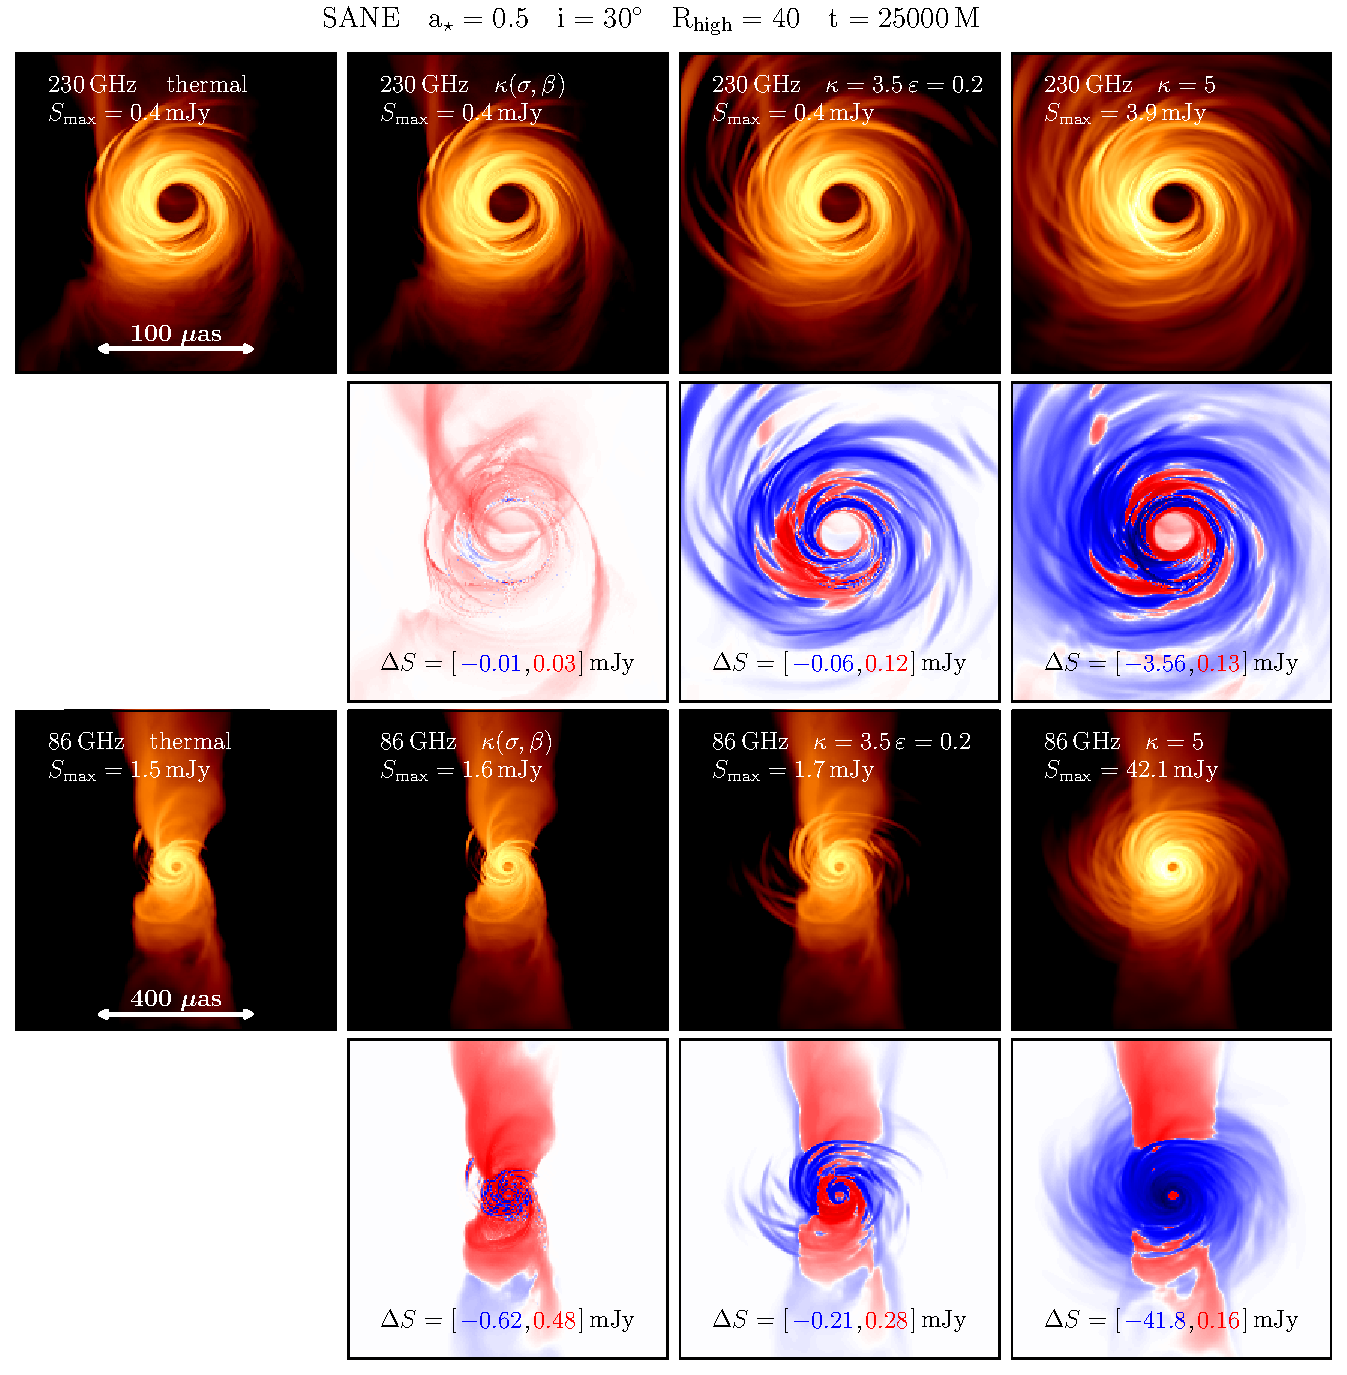
\includegraphics[width=\textwidth]{./figures/SANE_eDFs_diff.pdf}
  \caption{Influence of the eDF on the image structure for a SANE model with spin $a_{\star}=0.5$ seen under a viewing angle of $30\degree$ using $\Rh = 40$ at $t = \no{25000}\,\tg$.
    In the first and third row the panels show the image structure from left to right a thermal, variable kappa $\kappa(\sigma,\beta)$, $\kappa=3.5$ (fixed) with efficiency $\varepsilon=0.2$ and $\kappa=5$ (fixed) everywhere eDF at 230\GHz and at 86\GHz.
    Notice the increased field of view for the 86\GHz images.
    The second and fourth row show the difference between thermal image and the different non-thermal eDFs.}
  \label{fig:SANE_edfs}
\end{figure*}

Next we consider a mixed thermal/non-thermal eDF, with the non-thermal component following the $\kappa$ DF with $\kappa = 3.5$.
At high frequency $\nu L_\nu \sim \nu^s$ with $s = 2 - \kappa/2 = 1/4$, similar to what is seen in $2.2\um$ flares \citep{2007ApJ...667..900H}.
For this model set the GRMHD simulations use \bhac and the imaging uses \bhoss.

The fraction of non-thermal electrons is assumed to depend on $\sigma$ and $\beta$.  The emissivity
\begin{equation}
  j_{\nu,\rm{tot}}=(1-\epsilon) j_{\nu,\rm{thermal}} + \epsilon j_{\nu, \kappa},
  \label{eq:kappaeff}
\end{equation}
where the non-thermal efficiency 
\begin{equation}
  \epsilon(\varepsilon,\beta,\sigma)=\varepsilon\,
  \left[1 - e^{-\beta^{-2}}\right]
  \left[1-e^{-(\sigma/\sigma_{\rm min})^2}\right].
  \label{eq:efficiencybetasigma}
\end{equation}
Evidently $\epsilon \rightarrow 0$ in the disk while $\epsilon \rightarrow \varepsilon$ in the jet.
Since we remove emission at $\sigma > \sigma_{\rm cut} = 1$ the non-thermal electrons are confined to the jet sheath.

We set $\sigma_{\rm min}=0.01$ and vary the base efficiency, $\varepsilon$ over 0.05, 0.1 and 0.2.
At each $\varepsilon$ we generate a model set spanning the same parameter space as the thermal models (see Table~\ref{tab:radiativemodels}) and normalize the accretion rate using the standard procedure (see Section~\ref{sec:models}).

The mass accretion rate required to obtain 2.4\Jy at 230\GHz only changes on average around 1.5\% as compared to the thermal models.
This small variation in the mass accretion rate reveals the fact that most of the emission at 230\,GHz is created from the thermal part of the hybrid eDF, consistent with the small fraction of non-thermal particles added ($\varepsilon=0.05$, $0.1$, and $0.2$).

%..............................................................................
\subsubsubsection{230\GHz size and light curve Variability}
\label{varkappa230}

The addition of non-thermal particles does not substantially affect the flux or size of the image at 230\GHz.

For MAD models, 230\GHz emission is mostly produced in the disk region (see \citetalias{M87PaperV} and Figure~8 in \citealt{Wong_2022} for a 3D rendering).
Thus, the images are unaffected by the non-thermal particles, which are located in the jet.

For SANE models, increasing $\Rh$ pushes the emission towards the jet sheath which increases the source size for high spins and large $\Rh$.
However, the effect of non-thermal particles on the image is minor, because most of the emission is still produced by thermal electrons with temperature set by the $\Rh$ prescription (compare first and third panel in top row of Figure~\ref{fig:SANE_edfs}).

The passing fraction for the 230\GHz image size is 98\%, independent of $\varepsilon$, consistent with the thermal models.
We find that the 47\% of the models are in agreement with the 230\GHz variability constraint.
This passing fraction is larger than for the thermal models (27\%), due to the shorter time window ($\no{5000}\,\tg$) considered for the non-thermal models in contrast to $\no{15000}\,\tg$ for the thermal ones.

%..............................................................................
\subsubsubsection{Visibility Amplitude Morphology}

%The null location and VA morphology constraint are obtained from the 230\GHz images.
Since 230\GHz images of the $\kappa=3.5$ models with variable efficiency are similar to the thermal models (see previous paragraph) the fraction of passing models for the VA morphology are comparable.
The three non-thermal models have an average passing fraction for the Null location of 80\% whereas 83\% of the thermal models pass.
The VA morphology constrain is fulfilled by 72\% of the models for both thermal and non-thermal eDF.

%..............................................................................
\subsubsubsection{M-ring fits}

Given that including non-thermal particles via the equations presented in Equation~\ref{eq:efficiencybetasigma} does not change the image structure and variability properties of the 230\GHz images the M-ring fits provide the same passing fractions for the diameter (65\%), width (22\%) and asymmetry (95\%).

%..............................................................................
\subsubsubsection{86\GHz source size and flux}

The 86\GHz source is only slightly affected by the addition of non-thermal particles as compared to the thermal models.
Only the SANE models with $\Rh \geq 40$ and $\abh > 0$ produce 86\GHz image sizes larger than the thermal SANE models.
This effect can be seen in  first and third panel in the bottom row of Figure~\ref{fig:SANE_edfs}.
Notice the increased flux density in the jet sheath in the difference image (blue color).
This trend increases with the efficiency and is reflected in the decreasing pass fraction: 56\% (for $\varepsilon=0.05,0.1$) and 55\% ($\varepsilon=0.2$) as compared to thermal models (59\%).
A similar trend is found for the 86\GHz flux density.
The non-thermal particles are mainly located in the jet and thus contribute to the 86\GHz flux.
Again, jet dominated high spin SANE models typically fail the 86\GHz flux constraint.
With increasing efficiency i.e.
adding more non-thermal particles the pass fraction decreases, with 67\%  at $\varepsilon=0.05$, 66\% passing at $\varepsilon=0.1$, and 63\% passing at  $\varepsilon=0.2$ compared to a pass fraction of
68\% for the thermal models.

%..............................................................................
\subsubsubsection{$2.2\um$ Constraint}

The $2.2\um$ flux density increases for all models.
For SANE models, except $\Rh=1$, the addition of non-thermal particles leads to over-production of $2.2\um$ photons.
For MAD models, all models over-produce at $2.2\um$ for $\varepsilon \ge 0.05$.
As noted above, $2.2\um$ emission is produced from the tail of the eDF.
The thermal eDF tail decreases exponentially, while the $\kappa$ eDF tail decreases as a power law, so the increase in $2.2\um$ flux density is unsurprising.
This is a general feature of the non-thermal models: $2.2\um$ observations sharply limit the allowed population of non-thermal electrons.

%------------------------------------------------------------------------------
\subsubsection{Variable \texorpdfstring{$\kappa$}{kappa} Model}

The high-energy variability observed in many astrophysical sources including the galactic center may be associated with
%could be explained by
magnetic reconnection.
% cfg 2/5: this seems like more detail than provided for the other models
%During the reconfiguration of the magnetic field topology energy stored in the magnetic field is diffused into the plasma leading to the heating and acceleration of particles and finally resulting in the development of a non-thermal tails in the electron distribution functions.
Particle-in-cell (PIC) simulations have found that the slope of the non-thermal tail depends on  $\sigma$ and $\beta$ \citep[see, e.g.,][]{2018ApJ...862...80B}.  Here we consider a $\kappa$ eDF model in which $\kappa$ and $w$ vary  following the prescription of \cite{2018ApJ...862...80B}:
\begin{align}
  \kappa &= 2.8 +0.7\sigma^{-1/2} + 3.7\sigma^{-0.19}\tanh{(23.4\,\sigma^{0.26}\beta)}, \label{eq:kappa}\\
  w      &= \frac{ \kappa -3 }{\kappa} \Theta_e.
\end{align}

We use emissivities and absorptivities from  \cite{2016ApJ...822...34P}, computed numerically for the interval $3 < \kappa \le 8$.
For $\kappa > 8$ we substitute a thermal eDF.
As in the fiducial models we turn off emission at $\sigma > 1$.

The variable $\kappa$ models are computed from \hamr and \bhac GRMHD models where the time windows
$(\no{30000}$--$\no{35000})\,\tg$ (\hamr) and
$(\no{25000}$--$\no{30000})\,\tg$ (\bhac) are used.
% cfg 2/5: too much detail
%For the radiative transfer \ipole is applied to the \hamr models and the GRRT code \bhoss is employed for the \bhac models.
%For both models an image is created every 10\,M and we iterate the mass unit to obtain an average flux of 2.4\Jy at 230\GHz.
%In order to obtain the X-ray luminosity of the models, the Monte Carlo radiative transfer code \grmonty is connected to the \hamr models.

We find that the mass accretion rate needed to obtain $\langle F_{230} \rangle = 230\GHz$ is on average 4\% larger than for the thermal models, and thus the variable $\kappa$ models have slightly higher optical depth.
%The required mass accretion rate to obtain 2.4\Jy increases on average by 4\% as compared to the thermal.
%The larger mass accretion rate increases the number density of electrons, $n_e$, and thus the variable kappa models are slightly optically thicker than the thermal models.

%..............................................................................
\subsubsubsection{230\GHz size}

The disk region is dominated by thermal electrons (i.e. large $\kappa$) while the jet sheath has the lowest $\kappa$.
Therefore, the 230\GHz source size of the variable $\kappa$ models is similar to the thermal ones and no difference in pass fraction is found.
98\% of both models are in agreement with the 230\GHz size estimate (see first and second panel in the top row of Figure~\ref{fig:SANE_edfs}).
% cfg 2/9: this is almost certainly due to the short duration of the models
%With a passing fraction of 30\% a slightly larger number of $\kappa$ models show the same light curve variability as the observations (27\% for thermal models).

%..............................................................................
\subsubsubsection{Visibility Amplitude Morphology}

For the null location of the variable $\kappa$ models we find no difference to their thermal counterparts and for both $\sim$80\% pass this constraint.
However, there is a clear discrepancy between the variable $\kappa$ and thermal models regarding the VA morphology.
Only 60\% of the $\kappa$ models pass the VA morphology constraint, in contrast to 72\% of the thermal models.

%..............................................................................
\subsubsubsection{M-ring fits}

The thermal and variable $\kappa$ models agree in the passing fraction for the m-ring diameter (66\%), m-ring width (22\%) and asymmetry (95\%).

%..............................................................................
\subsubsubsection{86\GHz source size and flux}

The pass fraction for the 86\GHz source size constraint are comparable for thermal (59\%) and variable $\kappa$ models (55\%).
Given that most of the variable $\kappa$ models are optically thicker than their thermal counterparts the 86\GHz flux is on average lower which increases the passing fraction from 68\% (thermal eDF) to 75\% (variable $\kappa$ eDF).

%..............................................................................
\subsubsubsection{$2.2\um$ Constraint}

Including non-thermal particles via the $\kappa$ eDF increases the 2.2\um flux as compared to the thermal eDF.  In our prescription $\kappa$ decreases (more high energy electrons) as $\sigma$ increases.  In MAD models $\sigma$ is systematically larger than in SANE models.  Consistent with this, we find that most of the MAD models fail the 2.2\um constraint whereas in SANE models $\kappa$ is large and the passing fraction for SANE models is almost indistinguishable from their thermal counterparts.
%On the other hand in the low magnetised SANE models Equation~\ref{eq:kappa} leads to large $\kappa$ values i.e., less high-energy electrons in the tail of the eDF.
%Therefore, the passing fraction for the SANE models is almost the same as for their thermal counter-parts.
In total 35\% of the variable $\kappa$ models pass the 2.2\um constraint compared to 55\% for models including only thermal particles.

%..............................................................................
\subsubsubsection{X-ray constraint}

%As mentioned earlier, for the \hamr models we computed the x-ray luminosity.
Including non-thermal particles via the variable $\kappa$ eDF reduces the pass fraction from 61\% (for thermal eDF) to 35\%.  The $\kappa$ eDF provides a larger population of seed photons in the NIR and at higher energies that can be boosted into the X-ray by a single scattering event.
% cfg 2/5: this may be wrong, in the sense that the power-law tail has small optical depth and thus cannot contribute much to Compton scattering.  It seems more likely that the power-law tail extends the synchrotron bump to higher energies, and those higher energy seed photons are then upscattered by *thermal* electrons into the X-ray.
%This behaviour is agreement with our expectations since the $\kappa$ eDF provides a larger reservoir of high energy electrons contributing to the up-scattering of photons.

%..............................................................................
\subsubsubsection{Trends across \bhac and \hamr models for variable $\kappa$ models}

For the variable $\kappa$ models we have redundant models from \bhac and \hamr (see Table ~\ref{tab:GRMHDmodels}).
%Given the different adiabatic indices used (see Table~\ref{tab:GRMHDmodels}) a direct comparison between the models is difficult.
Both models sets show similar trends for all constraints (see Table~\ref{tab:passfraction}).
%, with the largest differences for the light curve variability and the VA morphology.
%For the \hamr models there is an increase of 21\% in the passing fraction for the light curve variability if non-thermal particles are included.
%Similar but not as pronounced for the variability constraint the fraction of passing models for the VA morphology increases from 39\% to 48\% if non-thermal particles are present.

%------------------------------------------------------------------------------
\subsubsection{Summary of Constraints on Non-Thermal Models}

\input{Tables/non-thermal_model_pass_fraction_table}

In Table~\ref{tab:passfraction} we list the pass fractions for \bhac and \hamr models using different eDFs.
Most non-thermal eDF models produce little change compared to the thermal models for most constraints.
The 86\GHz size and flux, which are the most important non-EHT constraints, are only marginally affected by the addition of non-thermal electrons.
This behaviour is obtained especially for eDFs which mainly add non-thermal particles in the jet while the disk is populated by thermal ones.
In our case this setup is given for variable $\kappa$ and $\kappa=3.5$ with variable efficiency and is consistent between \bhac and \hamr models (see Table~\ref{tab:passfraction}).

If non-thermal particles are included also in the disk, either via a power-law with slope p=4 stitched to a thermal distribution or via a $\kappa=5$ distribution, then there are some variations in pass fractions as compared to the above-mentioned eDFs.  For the power-law models the addition of non-thermal electrons increase the 86\GHz size by an average of 50\%.
However the pass fractions with respect to the thermal models is not changed.
In contrast the $\kappa=5$ model pass fractions decrease by 20\% compared to the thermal models.
For $p=4$ and $\kappa=5$, fewer models pass the 230\GHz m-ring width, with a consistent decrease by $\sim20\%$ for both models.
Interestingly the other m-ring constraints i.e., the diameter and asymmetry, are not affected by the addition of non-thermal particles.
This can be explained by the finer and brighter ring feature found in $p=4$ and $\kappa=5$ models connected to their smaller optical depth compared to their thermal counter-parts (see Table~\ref{tab:passfraction}).

In general the fraction of models passing $\mi{3}$ increases with the addition of non-thermal particles, independent of the prescriptions of the eDF.  This is due to the shorter duration of the exploratory runs and not an actual reduction in variability.   The main characteristic of the non-thermal models is the increase of 2.2\um and X-ray flux densities. However, in a large fraction of models this leads to overproduction of 2.2\um or X-ray flux and the pass fractions are reduced.

\begin{deluxetable*}{l|ccccc}\label{tab:fail_none}
\tablecaption{Exploratory models that pass all constraints}
\tablehead{
\colhead{Code/Setup} &
\colhead{MAD/SANE} &
\colhead{spin} &
\colhead{inc} &
\colhead{$\Rh$} &
\colhead{Constraint(s) failed at $15,000\tg$}
}
\startdata
\bhac $\kappa(\sigma, \beta)$	&	MAD		&	0.5		&	10		&	80 		& 	Mring width, \mi{3}		\\ 
\bhac $\kappa(\sigma, \beta)$	&	MAD		&	0.5		&	10		&	160		&	Mring width, \mi{3}		\\ 
\bhac $\kappa(\sigma, \beta)$	&	MAD		&	0.5		&	30		&	160		&	\mi{3}					\\ 
\hline
\bhac $\epsilon = 0.05$			&	SANE	&	0.94	&	10		&	10 		& 	\mi{3}					\\	
\hline
\hamr $p = 4$	  				&	SANE	&	0.94	&	50		&	40 		& 	2.2\,$\mu$m flux		\\	
\hamr $p = 4$	  				&	MAD		&	0.5		&	50		&	1 		&  	Mring diameter, \mi{3}
\enddata
\tablecomments{Exploratory models which pass all constraints when computed to $5,000\tg$. When extended to $15,000\tg$, each model fails one or more constraints. }

\end{deluxetable*}




Six non-thermal models pass all 11 constraints (see Table~\ref{tab:fail_none}).
These models are:
one \hamr MAD $p=4$ model with $\abh=0.5$ seen under an inclination $i=50\degree$ and
$\Rh=1$ and a high spinning SANE model with $\abh=0.94$ at an inclination of $i=50\degree$ with $\Rh=40$.
From the \bhac variable $\kappa$ three models are in agreement with all constraints namely: spin $\abh=0.5$ at inclination $i=10\degree$ at $\Rh=80$ and 160 and a model with the same spin seen under a slightly larger angle of $i=30\degree$ with $\Rh=160$.
The last of the six survivors is a \bhac SANE model with variable efficiency of $\varepsilon=0.05$ with an inclination of 10$^\degree$ and a $\Rh=10$.
These models share a common low inclination angle $i \leq 60\degree$ and positive spin.
We note that the MAD models coincide with the cluster of thermal models found for both \bhac and \kharma models (see Section~\ref{sec:summarythermal}).

\input{Tables/fail_one_non-thermal}

% cfg 2/5: this seems unnecessary
%The non-thermal models are run for only $\no{5000}\,\tg$, so most  constraints can not be applied as precisely.
%For example, the model distribution of $\mi{3}$ contains only $9$ points and is correspondingly more uncertain than for the thermal models.
%It is therefore difficult to detect subtle changes in models.

%==============================================================================
\subsection{Tilted Models}

Aligned models are a special case: in general one expects that the spin angular momentum of the black hole and the orbital angular momentum of the accretion flow are misaligned.
Here we consider misaligned flows around an $a_*=15/16$ black hole from \citet{Liska2018} and \citet{Chatterjee2020}.

All aligned models considered so far produce either a SANE or MAD accretion flow.
The tilted disk model initial conditions, however, produce a strongly magnetized near-MAD outcome with dimensionless magnetic fluxes between 25--50, a state we describe as  IN-SANE.
We consider three GRMHD simulations with tilt $0\degree$, $30\degree$ and $60\degree$.

The tilted models exhibit a warped disk due to  Lense-Thirring precession.
The time-averaged disk and jet are therefore non-axisymmetric.
Since the inner and the outer disk have different orientations, it is necessary to specify the coordinate axis of the observer.
We consider three  observer inclinations with respect to the {\em outer} disk at a single azimuth of $0\degree$ \citep[for more details, see][]{Chatterjee2020}.\footnote{A full parameter survey would run over azimuth angle as well.}

The 230\GHz pre-image size of edge-on large $\Rh$ models  increases slightly for the tilt-$60\degree$ compared to the aligned case.
This occurs because the inner jet is warped and creates an extended image.
This effect is also seen in the 86\GHz image size.
On the other hand, the 86\GHz flux varies little with tilt despite the presence of a boosted jet component at large tilt angles.

Variability increases with tilt.
In tilted disks, accretion occurs via thin plunging streams \citep[e.g.,][]{Fragile2007} where electrons in the shocked flow can be heated to relativistic temperatures \citep[e.g.,][]{Dexter2013, 2014ApJ...780...81G, White2019}, forming localized, fluctuating hotspots more easily than in aligned disks and increasing flux variability \citep{Chatterjee2020, 2021arXiv210412896W}.  Nevertheless, 20/27 models pass the \mi{3} constraint because of the short duration of the tilted models, which provide fewer \mi{3} samples than the fiducial models.

The $2.2\um$ flux density also increases with tilt.
The $2.2\um$ flux exceeds the 1.0\,mJy limit for all 3 tilts, with a few exceptions, e.g., $\Rh=160$ models at $10\degree$ inclination, which makes it difficult to favor the aligned case over the tilted one.
Furthermore misalignment destroys the axisymmetric nature of the accretion flow.
The current model set covers a small parameter space in inclination and $\Rh$.
A thorough exploration of the source azimuthal angle with respect to the observer is left to future studies.

To summarize: for the model set considered here tilt primarily affects variability and the $2.2\um$ flux density, tending to increase both and thus shifting acceptable aligned models into rejected models as tilt angle increases.
These trends are consistent with those observed by \cite{2021arXiv210412896W}.

%==============================================================================
\subsection{Stellar Wind Fed Models}

The accretion models of \cite{2020ApJ...896L...6R, 2020MNRAS.492.3272R, 2018MNRAS.478.3544R} track plasma from  magnetized stellar winds down to the event horizon and provide a self-consistent picture of the origin of both gas and magnetic fields in the accreting plasma in \sgra.
The resulting inflow does not fully circularize, so the models provide a distinct alternative to the fiducial models, which {\em assume} that the torus initial conditions relax to an astrophysically accessible state for the inner accretion flow.
In the wind-fed models the density of the wind is fixed, so the 230\GHz flux density is matched to observations by varying $\Rh$ instead.

We use two versions of the model: one in which the stellar wind magnetization is low ($\beta = 10^6$) and a second in which the magnetization is high ($\beta = 10^2$).
$\Rh$ is adjusted until each model has the observed time-averaged 230\GHz flux density, with $\Rh = 13$ ($\beta = 10^6$) and $\Rh = 28$ ($\beta = 10^2$).

Both wind-fed models produce rings that are too narrow, failing the \mring width test.
In addition both are too bright at 86\GHz and fail the $\mi{3}$ test, although they are quieter than MAD models and close to the cutoff.

Both non-EHT and EHT constraints have the power to test wind-fed models.
It is {\em not} possible to draw broad conclusions about the viability of the wind-fed models in general, however, since the two models tested here contain only a single spin ($\abh=0$) and all use the $\Rh$ thermal eDF model.
